% !TEX TS-program = pdflatex
% !TEX encoding = UTF-8 Unicode

% This is a simple template for a LaTeX document using the "article" class.
% See "book", "report", "letter" for other types of document.

\documentclass[11pt]{report} % use larger type; default would be 10pt

\usepackage[utf8]{inputenc} % set input encoding (not needed with XeLaTeX)

%%% Examples of Article customizations
% These packages are optional, depending whether you want the features they provide.
% See the LaTeX Companion or other references for full information.

%%% PAGE DIMENSIONS
\usepackage{geometry} % to change the page dimensions
\geometry{a4paper} % or letterpaper (US) or a5paper or....
% \geometry{margin=2in} % for example, change the margins to 2 inches all round
% \geometry{landscape} % set up the page for landscape
%   read geometry.pdf for detailed page layout information

\usepackage{graphicx} % support the \includegraphics command and options

% \usepackage[parfill]{parskip} % Activate to begin paragraphs with an empty line rather than an indent

%%% PACKAGES
\usepackage{booktabs} % for much better looking tables
\usepackage{array} % for better arrays (eg matrices) in maths
\usepackage{paralist} % very flexible & customisable lists (eg. enumerate/itemize, etc.)
\usepackage{verbatim} % adds environment for commenting out blocks of text & for better verbatim
\usepackage{subfig} % make it possible to include more than one captioned figure/table in a single float
\usepackage{hyperref}
% These packages are all incorporated in the memoir class to one degree or another...

%%% HEADERS & FOOTERS
\usepackage{fancyhdr} % This should be set AFTER setting up the page geometry
\pagestyle{fancy} % options: empty , plain , fancy
\renewcommand{\headrulewidth}{0pt} % customise the layout...
\lhead{}\chead{}\rhead{}
\lfoot{}\cfoot{\thepage}\rfoot{}

%%% SECTION TITLE APPEARANCE
\usepackage{sectsty}
\allsectionsfont{\sffamily\mdseries\upshape} % (See the fntguide.pdf for font help)
% (This matches ConTeXt defaults)

%%% ToC (table of contents) APPEARANCE
\usepackage[nottoc,notlof,notlot]{tocbibind} % Put the bibliography in the ToC
\usepackage[titles,subfigure]{tocloft} % Alter the style of the Table of Contents
\renewcommand{\cftsecfont}{\rmfamily\mdseries\upshape}
\renewcommand{\cftsecpagefont}{\rmfamily\mdseries\upshape} % No bold!

%%%Chapter style
\usepackage[explicit]{titlesec}
\usepackage{lmodern}
\usepackage{lipsum}

\newlength\chapnumb
\setlength\chapnumb{4cm}

\titleformat{\chapter}[block]
{\normalfont\sffamily}{}{0pt}
{\parbox[b]{\chapnumb}{%
   \fontsize{120}{110}\selectfont\thechapter}%
  \parbox[b]{\dimexpr\textwidth-\chapnumb\relax}{%
    \raggedleft%
    \hfill{\LARGE#1}\\
    \rule{\dimexpr\textwidth-\chapnumb\relax}{0.4pt}}}
\titleformat{name=\chapter,numberless}[block]
{\normalfont\sffamily}{}{0pt}
{\parbox[b]{\chapnumb}{%
   \mbox{}}%
  \parbox[b]{\dimexpr\textwidth-\chapnumb\relax}{%
    \raggedleft%
    \hfill{\LARGE#1}\\
    \rule{\dimexpr\textwidth-\chapnumb\relax}{0.4pt}}}
    
\setlength{\parindent}{2em}
\setlength{\parskip}{1em}

%%%pseudo-code 
\usepackage{amsmath}
\usepackage{algcompatible}
\usepackage{algorithm}
\usepackage{algorithmicx}
\usepackage[noend]{algpseudocode}
%\usepackage[]{algorithm2e}
\makeatletter
\def\BState{\State\hskip-\ALG@thistlm}
\makeatother

\graphicspath{ {imgs/} }
\usepackage[tc]{titlepic}

%datetime
\usepackage[UKenglish]{datetime}
\newdateformat{mydate}{\monthname[\THEMONTH] \THEYEAR}
%%% END Article customizations

%%% The "real" document content comes below...
\begin{document}
\begin{titlepage}
\begin{center}

%\begin{minipage}[r]{0.5\textwidth}
%
\includegraphics[width=\textwidth]{rml_logo}
%\end{minipage}

%\begin{minipage}[r]{0.5\textwidth}
\textsc{\Large University Bordeaux 1}\\
%\end{minipage}
%\end{center}
%\begin{flushleft}
\vspace{10mm}
\textit{ Internship report - Master Informatics in Software Engineering}
%\end{flushleft}

\vspace{4mm}
\hrule height 1mm
\vspace{0.5mm}
\hrule
\vspace{1mm}
\textbf{\LARGE \textsc{Internship at Rainmaker Labs}}
\vspace{4mm}
\hrule \vspace{0.5mm}
\hrule height 1mm

\vspace{10mm}

\textsc{By}\\
\vspace{1mm}
\textsc{Quang Anh NGUYEN}\\
\vspace{10mm}

\textsc{Department of Informatics}\\
\textsc{University Bordeaux 1}




%\vfill
\vspace{15mm}

\mydate\today
%\maketitle
\end{center}
\end{titlepage}

%\date{} % Activate to display a given date or no date (if empty),
         % otherwise the current date is printed 



\newpage
\begin{center}
{\huge Abstract}
\end{center}

Mobile development is one of the most popular industries nowaday. Each year there are several hundreds millions of smartphones which were sold, in which Android devices and iOS devices hold the most part, around 98\% of the market. I decided to learn about Android development, since it used Java language, the most familiar programming language to me. For that reason I applied into a branch of Rainmaker Labs in Vietnam, a mobile development outsourcing company.
\newpage
\newpage
\tableofcontents
\listoffigures

\chapter{Acknowledgement}

I would like to express my gratitude to Mr. Tran Tan Phong, for allowing me join in the company, although I didn't have any experience in the field I applied for. I also would like to express my gratitude to Mr. Tran Thanh Tri, Mr. Pham Tien Vinh, tech leader and project leader, for training me and helping me understand many technical problems. To Mr. Le Vuong Thien, project manager, who helped me getting familiar with SCRUM method. 

%%%chapter 1
\chapter{Introduction}
\section{Rainmaler Labs}

Rainmaker Labs is the singaporean outsourcing company, specialized in mobile development, currently placed first among the competitors in Singapore and Asia Pacific. 

Rainmaker Labs in Vietnam is the new branch which was established in Feb 2015. Though it's new, but thanks to the politics, cultures and remuneration policy, the offshore branch was able to recruit many talented and experienced individuals, some of them even hold high position in their previous jobs.

\section{Projects}

Although I was new to Android at that time, infact, I had never touch Android before, but I still managed to convince my seniors to let me participate in company's projects. The first project was the small project, named \textbf{Pedro}, which served at the \textbf{Charle \& Keith Fasionable Awards 2015}. In this project I was able to study about the basic of Android development and some advanced technic.

The second one is a big project. This project is the digital version of Singapore government project, \textbf{Electronic Tourist Refund Scheme} aka \textbf{eTRS}. In this report I will concentrate on the technics, and knownledge which I was able to acquired. 


%%%chapter 2
\chapter{Software Development Method}

In Rainmaker Labs, we use \textbf{SCRUM} as our software deployment method. With this method, we could deploy software to the customer as fast as possible, and be closest to customer's expectation. There are some important points such as :

\begin{itemize}
	\item break down the project into small tasks, as small as possible.
	\item estimate the difficulties of each task and give points to them, then each member of team will select their task, base on their capability, such that all the team members have the same amount of points.
	\item during the development process, whenever a member encounter a problem which he couldn't solve, they could always ask for help. Team leader, or someone else who did solve the problem before could give hints to help him resolve his issue.
	\item everyday before starting working, team will have a stand-up meeting for about 10 minutes. Scrum master would hear team member reporting about their processes the previous day, and their planning for today's works. 
	\item after each sprint (about a week), team will demonstrate what they have done to the client, allowing them to follow the development process, and correct the features to their ideal.
	\item after some sprints, when the product is about to finish, the tester team will join and dug in for bug. The development team now will start to fix the reported bug, along with working on their tasks.
\end{itemize}

%%%chapter 3
%\chapter{How I understand about Android development}

Although Android use Java as its programming language, writing an Android application is more complicated than writing a Java one.

\section{Activity and Fragment}

\subsection{Activity}
One of the most important component in Android is \textit{Activity}. An \textit{Activity} represent a screen in an application, and an instance of this kind of class is not initialized by user, infact, it is created by the Android's system, by injection via a file \textit{manifest.xml}. For that reason, transfer data between \textit{Activities} can't be done by the usual ways. Using static variable is no good neither, because each \textit{Activity} has their own life circle, when its life circle ends, the system will kill the \textit{Activity}, and garbage collector will free the memory zone which was hold by this \textit{Activity}, that makes all the static variables reset. 
\subsection{Fragment}
A \textit{Fragment} is a portion of an \textit{Activity}, it could be added or removed when an \textit{Activity} is active. A \textit{Fragment} also has its own life circle.

%%%chapter 4
\chapter{My Project}

\section{Project's purpose}\label{condition}

\textbf{Electronic Tourist Refund Scheme} (ETRS) is a government's project, which allowed the tourists who visit Singapore could reclaim Good and Service Tax if he bought a product in Singapore.

To be able to reclaim the refund money, a condition have to be satisfied: 
\begin{itemize}
	\item receipt's value must exceed 100 SGD
	\item merchant or shop who generated the receipt must registry for the ETRS project
	\item if receipt's value don't exceed 100 SGD, it could be grouped with maximum another 2 receipts, such that the total value of this group must exceed 100 SGD and all the receipts within this group must belong to the same merchant or shop
\end{itemize}



Our job is to realize the idea of the ETRS project into mobile device. 

\section{Important technics implemented}

\subsection{BlinkID}
BlinkID is a library allow scanning the passport of tourist. From the information we got from the scan, we can create account for the tourist, thus each person is associated with his/her passport. So even if a tourist lost his account, the refund process still could going on if he still keep his passport.

\subsection{QR code}
Each tourist, after registry their account, is given 1 QR code. In case that he don't want to show his passport, he could use this QR code to identify himself. Each merchant or shop would have their own QR code, and the tourist can scan their QR code for the ID of the shop.

\subsection{Android location service}
Using this service, the application will notice the tourist if he's near one of the shop registry for the ETRS project. This service locates the user's position either by wifi or by GPS.

\subsection{Geofencing}
This function allow the application to detect if the user is going in or out of the airport, thus allow to take correspondant behavior.

\subsection{Push notification}
This allows the server to notify users when there're change in their data, such as if their request to refund is realized, or refused. 

\subsection{Google Cloud Message (GCM)}
The application allow user to define their events that need to be notified when the time come, for example the flight's time. Application will use GCM to notify the user when such time come.

\subsection{Social network sharing}
The application allow user to share on their social network, such as Facebook, Wechat, Sina Weibo. And this is abig challenge, because China's social network (Wechat, Sina Weibo) do not have many tutorials in English, and the procedure to register application ID on these network is complicated too. 

\subsection{Map}
Google Map service is intergrated into the application, thanks to the need of path finder. It's not very complicated, but then the problem rise. As Google Map can't be used inside China, we have to adopt another map service from China, Baidu map, and this process is extremely difficult, from the registration process to implementation process, since this service only work if you are in China, even fake GPS couldn't help.


\section{Algorithm utilized}

I was given the task to write the algorithm that filter a list of receipts and return receipts which satisfy the condition in  \ref{condition}. 

\subsection{Brief description}
Given the list of receipts, could be generated by many shops, extract a list of receipts which satisfy the conditions in \ref{condition}.

\subsection{Solution}
We devide the list of receipts into many lists such that the receipts in each list belong to one shop only. This lead to a new problem: 
Given the list of receipts, all receipts belong to 1 shop, extract a list of receipts which satisfy the condition in \ref{condition}

\subsubsection{Step 1}
Extract all the receipts which value greater or equal 100. Then sort the rest of list in increased order.

\subsubsection{Step 2}
Divide the ordered list into many smaller lists :

\begin{algorithm}[H]
\caption{Split list of receipts into many sublists}
\begin{algorithmic}
\Function{SplitList}{receipts}
\State $j = 0, i = 0$
\While{$i < \textit{receipts}.length$}
\If {$\Big[ \cfrac{\textit{receipts}[i].value}{10} \Big]  \leq  j$}
	\State $list_{j}.add(\textit{receipts}[i])$
	\State $i++$.
\Else
	\State $j++$
\EndIf
\EndWhile
\EndFunction
\end{algorithmic}
\end{algorithm}

\subsubsection{Step 3}
From the sublists, we will extract groups of receipts which satisfy the condition. There's some preconditions we could make for simplifier the process.

\begin{itemize}
\item for a group of 2 receipts, if they belong to $list_{i}$ and $list_{j}$ then $i+j \geq 9$
\item for a group of 3 receipts, if the belong to $list_{i}$, $list_{j}$ and $list_{k}$ then $i+j+k \geq 8$
\end{itemize}


First of all we need a function that check the condition of a set of receipt. If satisfy, remove the receipts from their correspondant sublist, and add a new group of receipt to our list of group and return true. Otherwise return false.

\begin{algorithm}[H]
\caption{Check if the correspondant receipts could form a group}
\begin{algorithmic}
\Function{Check}{i, j, k, a, b, c, groups}

\State $r_{a} = list_{i}[a]$
\State $r_{b} = list_{j}[b]$
\State $r_{c} = list_{k}[c]$

\If{$r_{a}.value + r_{b}.value \geq 100 \land (i \neq j \lor a \neq b)$}
	\State groups.add(\textbf{new} Group($r_a, r_b$))
	\State $list_i.remove(r_a), list_j.remove(r_b)$
	\State \Return{true}
\EndIf

\If{$r_{b}.value + r_{c}.value \geq 100 \land (j \neq k \lor b \neq c$}
	\State groups.add(\textbf{new} Group($r_b, r_c$))
	\State $list_j.remove(r_b), list_k.remove(r_c)$
	\State \Return{true}
\EndIf

\If{$r_{a}.value + r_{c}.value \geq 100 \land (i \neq k \lor a \neq c)$}
	\State groups.add(\textbf{new} Group($r_a, r_c$))
	\State $list_i.remove(r_a), list_k.remove(r_c)$
	\State \Return{true}
\EndIf

\If{$r_a.value + r_b.value + r_c.value \geq 100 \land (i \neq j \lor a \neq b) \land (i \neq k \lor a \neq c) \land (j \neq k \lor b \neq c)$}
	\State groups.add(\textbf{new} Group($r_a, r_b, r_c$))
	\State $list_i.remove(r_a), list_j.remove(r_b), list_k.remove(r_c)$
	\State \Return{true}
\EndIf

\Return{false}
\EndFunction
\end{algorithmic}
\end{algorithm}

The next function is the main one that extract a list of groups of receipts from the sublists.

\begin{algorithm}[H]
\caption{}
\begin{algorithmic}[1]
\Function{Filter}{}
\State $i=0, j=0, k=0$
\State groups
\State \underline{loop\_i}:
\For{$i=0$ \textbf{to} $9$}
	\State $a=b=c=0$
	\While{$a < list_i.size$}
	\State \underline{loop\_j}:
	\For{$j=i$ \textbf{to} $9$}
		\State $b=c=0$
		\While{$b < list_j.size$}
		\State \underline{loop\_k}:
		\For{$k=j$ \textbf{to} $9$}
			\State $c=0$
			\While{$a < list_i.size \land b < list_j.size \land c < list_k.size$}
				\If{$i=j$}
					\If{$a=b$}
						\If{$i+k \geq 9$}
							\If{$j \neq k \lor a \neq c$}
								\If{$\neg \Call{Check}{i,j,k,a,b,c,groups}$}
									\State $c++$
								\EndIf
							\Else
								\State $c++$
							\EndIf
						\Else
							\State \textbf{goto} \underline{loop\_k}
						\EndIf
					\Else % a!=b AND i=j
						\If{$k=j \land (c=a \lor c=b)$}
							\If{$i+j \geq 9$}
								\If{$\neg \Call{Check}{i,j,k,a,b,c,groups}$}
									\State $c++$
								\EndIf
							\Else
								\State \textbf{goto} \underline{loop\_k}
							\EndIf						
						\Else
							\If{$\neg \Call{Check}{i,j,k,a,b,c,groups}$}
								\State $c++$
							\EndIf
						\EndIf
					\EndIf
				\Else % i!=j break into page 2 here
				\algstore{filterbreak}
				\end{algorithmic}
				\end{algorithm}
				
				\begin{algorithm}
				\begin{algorithmic}
				\algrestore{filterbreak}
					\If{$j=k$}
						\If{$b=c$}
							\If{$\neg \Call{Check}{i,j,k,a,b,c,groups}$}
								\State $c++$
							\EndIf
						\Else
							\If{$i+j+k \geq 8$}
								\If{$\neg \Call{Check}{i,j,k,a,b,c,groups}$}
									\State $c++$
								\EndIf
							\Else
								\State \textbf{goto} \underline{loop\_k}
							\EndIf
						\EndIf
					\Else % j!=k
						\If{$i+j+k \geq 8$}
							\If{$\neg \Call{Check}{i,j,k,a,b,c,groups}$}
								\State $c++$
							\EndIf
						\Else
							\State \textbf{goto} \underline{loop\_k}
						\EndIf
					\EndIf
				\EndIf
			\EndWhile
		\EndFor
		\State $b++$
		\EndWhile
	\EndFor
	\State $a++$

	\EndWhile
\EndFor
\State \Return{groups}
\EndFunction
\end{algorithmic}
\end{algorithm}



\chapter{Knowledge acquired}

During the time of this project, I have learnt many things, from non-technical to technical, such as teamwork, communication, code re-used, code convention. 

\section{Design Pattern}

Code re-used is an important factor in software development industry. You can work faster or not depends on how good your code re-using skill is. And design pattern is a part of code re-used. In the project, there are some views that were used in many screens. At first I repeat the same implementing process everytime, and the code for each screen grow quite big. That's when I started to use design pattern, and suprisingly, it work well.


\begin{figure}[H]
\centering
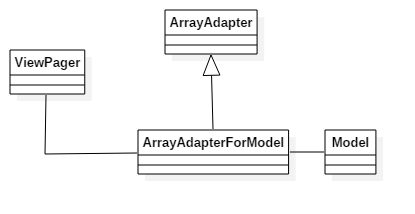
\includegraphics[scale=0.7]{ClassDiagram1}
\caption{Class diagram for normal use of ViewPager}
\end{figure}

\textit{ViewPager} is a view provided by Android, it's used to perform slide action when there'are many images, or sections. Above is a class diagram when normally implementing ViewPager. An instance of \textit{Model} is a data object that we want to present it within \textit{ViewPager}. So if we have many class \textit{Models}, we have to rewrite \textit{ArrayAdapter} corresponding to each \textit{Model}. So my first approach is below :

\begin{figure}[H]
\centering
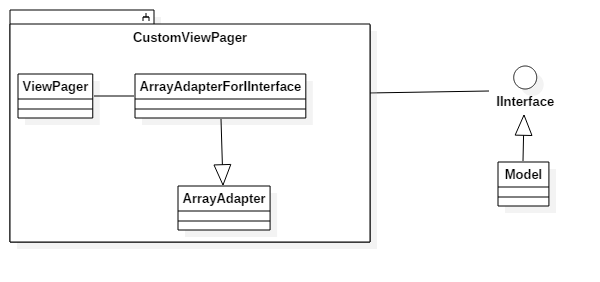
\includegraphics[scale=0.7]{ClassDiagram2}
\caption{First approach}
\end{figure}

With this approach, my code reduce significantly. I just have to write some more functions defined in \textit{IInterface} for \textit{Model}. But then there's another problem. I have to rewrite some classes \textit{Model} that I had created long before, and everyone were working on it, so modifying existed file need to be prevented. Then I came up with second approach, based on the first one :

\begin{figure}[H]
\centering
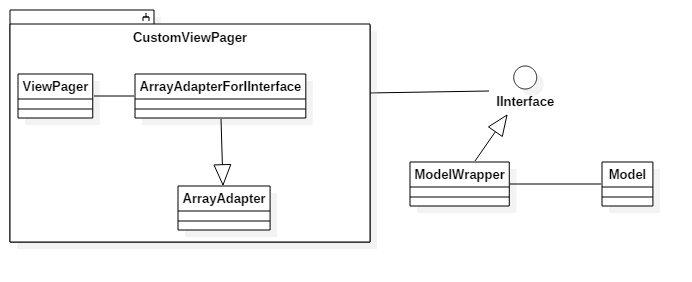
\includegraphics[scale=0.7]{ClassDiagram3}
\caption{Second approach}
\end{figure}

This time, instead of extending class \textit{Model}, I used a medium \textit{ModelWrapper} which envelop \textit{Model} and implement interface \textit{IInterface}. Then each time I want to apply \textit{CustomViewPager} for a new \textit{ModelA}, I just need to create a class \textit{ModelAWrapper} (normally this wrapper had around 20 lines of code).

And after reviewing this scheme, I just realized that I had just apllied \textit{Adapter Pattern} in \textit{Design Pattern}.

\section{Custom View}

Apart from \textit{Design Pattern}, making custom view and re-used it is a great way of re-using code too. In this project, I had made a textview in which the text is align with the diagonal of the textview's bound, a circle view which has shadow, and a layout with shadow. 

Custom component could make your work easier, depend on how convenient it became. In Android, a \textit{Spinner} is a dropdown combo box, which let user choose an item from its dropdown list. The normal way of using such component, is to enter a list of \textit{String}, and when user choose one item, this \textit{Spinner} will return the position of the selected item, and then we can retrieve the corresponding object. 

\begin{figure}[H]
\centering
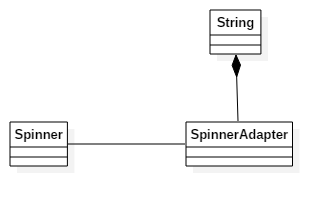
\includegraphics[scale=0.7]{Spinner1}
\caption{Tradition Spinner}
\end{figure}

Let analize the example below :

I have an array of \textit{Good}, like Candy, Wine, Clothes, etc. If I want to make a \textit{Spinner} using the above method to display good's name, and available quantity, it would be a little more complicated, since each item has 2 values: a name, and a quantity number, but it's still doable. Then if we want to add more functions, such as reduce the quantity, it would mean that we have to clear the data of the \textit{Spinner}, and re-insert the new data each time we updated the data. 

So I came up with another solution. Instead of using the tradition \textit{String} as input for \textit{Spinner}, I decide to use \textit{Good}. And every time an instance of \textit{Good} is updated, its automatically update the \textit{Spinner} as well. And moreover, when I selected an item in the dropdownlist, unlike before, I obtain a \textit{Good}'s instance, instead of a \textit{String}. And that make my work faster and easier. 

\begin{figure}[H]
\centering
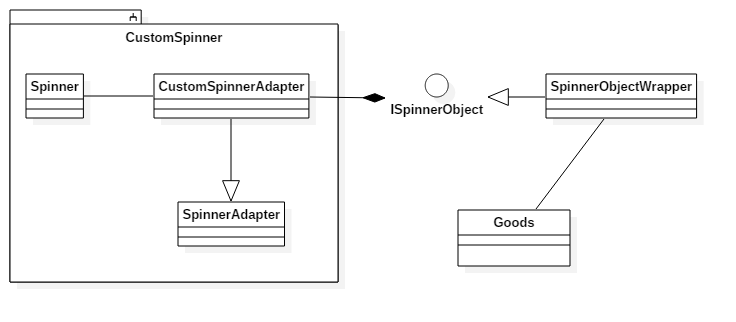
\includegraphics[scale=0.7]{Spinner2}
\caption{My Spinner}
\end{figure}
\chapter{Conclusion}

Thanks to my job in Rainmaker Labs, I came to understand the development procedure, from scratch to finish. I was able to make acquaintance with SCRUM method. I had chances to aplly my university's knowledge, such as algorithm, design pattern, and for that reason, I actually could understand them more than before. I also could analyze a problem by looking it from many perspectives. I was able to learn about Android development, and have a broader view on mobile development (both Android and iOS).

I had chance to experience teamwork in a big group doing a big project. I made acquaintance with many colleagues, and learned a lot from them, since I'm more theoretical than practical. These relationships and knowledge will help me alot in my future career. 

\end{document}